\documentclass{beamer}

\usepackage[english]{babel}
\usepackage{beamerthemeBoadilla}
%\usepackage{beamerthemeCambridgeUS}
%\usepackage{beamerthemeRochester}
%\usepackage{beamerthemeSzeged}
%\usepackage{beamerthemeMontpellier}
%\usepackage{beamerthemedefault}
\usepackage{url}
\usepackage{verbatim}
\usepackage[utf8]{inputenc}
\usepackage{multirow}
\usepackage{fancyvrb}
\usepackage{proof-dashed}
\newcommand{\mz}{\m{match} \;}
\newcommand{\stepz}{\m{step} \;}
\newcommand{\tab}[0]{\;\;\;\;}
\newcommand{\dz}{\m{derive}~}
\newcommand{\comp}[0]{\m{comp} \;}
\newcommand{\az}{\m{apply} \;}
\newcommand{\doz}{\m{run} \;}
\newcommand{\seqnocut}[3]{#1 ; #2 \Rightarrow #3}
\newcommand{\defeq}{\buildrel\triangle\over =}
\newcommand{\compr}[1]{\m{def} \; #1}

\newcommand{\stepo}{\m{step}_{LLD} \;}
\newcommand{\mo}{\m{match}_{LLD} \;}
\newcommand{\contlld}{\m{cont}_{LLD}}
\newcommand{\cont}{\contlld \;}
\newcommand{\contclld}{\m{cont}_{LLDc}}
\newcommand{\contc}{\contclld \;}
\newcommand{\done}{\m{derive}_{LLD} \;}
\newcommand{\doo}{\m{run}_{LLD} \;}
\newcommand{\matchlldc}{\m{match}_{LLDc}}
\newcommand{\mc}[0]{\matchlldc \; }
\newcommand{\dall}[0]{\m{fix}_{LLD} \; }
\newcommand{\strans}[0]{\m{update}_{LLD} \;}
\newcommand{\dc}{\m{derive}_{LLDc} \;}
\newcommand{\ao}{\m{apply}_{LLD} \;}

\newcommand{\com}{\xrightarrow{*}}
%\mapsto}
\newcommand{\feq}[2]{#1 \equiv #2}
\usepackage{latexsym}
\usepackage{amssymb}            % for \multimap (-o)
\usepackage{stmaryrd}           % for \binampersand (&), \bindnasrepma (\paar)

\newcommand{\m}[1]{\mathsf{#1}}
\newcommand{\f}[1]{\framebox{#1}}

\newcommand{\eph}{\mathit{eph}}
\newcommand{\pers}{\mathit{pers}}
\newcommand{\um}[1]{\underline{\m{#1}}}

\newcommand{\seq}{\vdash}
\newcommand{\semi}{\mathrel{;}}
\newcommand{\lequiv}{\mathrel{\dashv\vdash}}

% symbols of linear logic
\newcommand{\lolli}{\multimap}
\newcommand{\tensor}{\otimes}
\newcommand{\with}{\mathbin{\binampersand}}
\newcommand{\paar}{\mathbin{\bindnasrepma}}
\newcommand{\one}{\mathbf{1}}
\newcommand{\zero}{\mathbf{0}}
\newcommand{\bang}{{!}}
\newcommand{\whynot}{{?}}
\newcommand{\bilolli}{\mathrel{\raisebox{1pt}{\ensuremath{\scriptstyle\circ}}{\lolli}}}
% \oplus, \top, \bot



\newsavebox{\mysavebox}

\def\Tiny{\fontsize{6pt}{6pt}\selectfont}

\title{A Linear Logic Programming Language for Concurrent Programming over Graph Structures}
\author[Flávio Cruz]{Flávio Cruz {\small \texttt{<fmfernan@cs.cmu.edu>}}\\
\scriptsize{\textbf{Authors}:\\
Flavio Cruz (CMU/UP)\\
Ricardo Rocha (UP)\\
Seth Goldstein (CMU)\\
Frank Pfenning (CMU)}}

\institute[CMU/UP]{Carnegie Mellon University \\ Pittsburgh, PA 15213, USA \and
CRACS \& INESC TEC, Faculty of Sciences, University Of Porto\\
Rua do Campo Alegre, 1021/1055, 4169-007 Porto, Portugal}
\date{\today}

\let\oldalert\alert
\renewcommand{\alert}[2][]{%
  \if\relax\detokenize{#1}\relax% http://tex.stackexchange.com/q/53068/5764
    \oldalert{#2}% Default overlay
  \else
    \oldalert<#1>{#2}% Specific overlay
  \fi}

\begin{document}

\frame{\titlepage}

\AtBeginSection[] { \begin{frame}<beamer>
\frametitle{Plan} \tableofcontents[currentsection]
\end{frame}}

\section{Motivation}

\frame
{
   \frametitle{The importance of graph-based algorithms}
   \begin{itemize}
      \item Graphs are a very general data structure that can represent anything
      \item The internet has become a huge source of graph-based data:
      \begin{itemize}
         \item Web pages
         \item Social networks
         \item Online databases (IMDB)
      \end{itemize}
      \item Frameworks for manipulating and analyzing graph data:
      \begin{itemize}
         \item GraphLab / PowerGraph: machine learning
         \item Pregel / Giraph (OSS): iterative scalable graph processing
         \item Ligra: graph processing in shared memory
      \end{itemize}
      \item Lack of practical logic-based approaches to tackle these problems
      \begin{itemize}
         \item Most of the solutions use imperative paradigms
         \item Advantages of logic solutions: declarative and amenable to proof
         \item Harder for designers to make it fast
      \end{itemize}
   \end{itemize}
}

\frame
{
   \frametitle{Logic and graphs}
   \begin{itemize}
      \item Declarative networking: P2
      \begin{itemize}
         \item Datalog-like language for developing network algorithms
         \item Rules are localized and logical facts are local to a node
         \item Execution: local computation + communication (messages)
      \end{itemize}
      \item Ensemble programming: Meld
      \begin{itemize}
         \item Inspired by P2, it was developed for programming ensembles of moving robots
         \item Innovation: logical facts for sensing and acting on the world
         \item Uses incremental evaluation and retraction to account for world changes (like P2)
      \end{itemize}
      \item \textbf{General graph-based programming: Linear Meld~(LM)}
      \begin{itemize}
         \item Language loosely based on Meld that uses Linear Logic as its foundation
         \item Mutable state can be expressed declaratively
         \item For general graph-based programming
         \item Retains sensing facts and action facts for improving program execution but that is not the aim of this talk
      \end{itemize}
   \end{itemize}
}

\section{Linear Meld}

\begin{frame}[fragile]
   \frametitle{Linear Meld: How does it work?}
   \begin{itemize}
      \item Forward-chaining linear logic programming
      \begin{itemize}
         \item We start with a set of rules and a database of logical facts
         \item The database of facts is used to apply more rules
         \item Program stops when no more information can be derived
      \end{itemize}
      \item Facts are also localized on a per-node basis
      \begin{itemize}
         \item Nodes can run with any order - no guarantees are given
         \item Rules are derived locally - no synchronization issues
      \end{itemize}
      \item Computation follows a don’t care or committed choice non-determinism
      \begin{itemize}
         \item Rules have a pre-defined priority: if there are enough facts, the rule with higher priority will run
      \end{itemize}
   \end{itemize}
\end{frame}

\subsection{Bipartiteness Checking}

\begin{frame}[fragile]
  \frametitle{Bipartiteness Checking}
  \begin{columns}[t]
     \column{.45\textwidth}
     \begin{block}{Program}
       \begin{Verbatim}[fontsize=\tiny,commandchars=\\\{\},frame=single]
\alert[1]{type route edge(node, node).}
\alert[1]{type linear mark(node, int).}
\alert[1]{type linear uncolored(node).}
\alert[1]{type linear colored(node, int).}
\alert[1]{type linear fail(node).}

fun next(int X) : int =
   if X <> 1 then 1 else 2 end.

\alert[2,6]{mark(@1, 1).}
\alert[2]{!edge(@1, @2). !edge(@1, @3).}
\alert[2]{!edge(@2, @4). !edge(@3, @4).}
\alert[2]{uncolored(A).}

\alert[3,7,8,9,10]{mark(A, P), uncolored(A)}
   \alert[3,7,8,9,10]{-o \{B | !edge(A, B) | mark(B, next(P))\},}
      \alert[3,7,8,9,10]{colored(A, P).}

\alert[4,11]{mark(A, P), colored(A, P)}
   \alert[4,11]{-o colored(A, P).}
\alert[5]{mark(A, P1), colored(A, P2), P1 <> P2}
   \alert[5]{-o fail(A).}
       \end{Verbatim}
     \end{block}
      \column{.5\textwidth}
      \begin{block}{\only<1>{Predicates}\only<2>{Axiom}\only<3>{First rule}\only<4>{Second rule}\only<5>{Third and fourth rule}\only<6-11>{Execution}}
         \centering
         {\scriptsize
         \only<1>{\begin{itemize}
                \item The first argument of every predicate must be typed as \texttt{node}.
                \item Predicates specified as \texttt{route} inform the compiler about the graph data structure.
                \item Predicates specified as \texttt{linear} turns facts of the predicate into linear facts, which can be asserted or retracted.
                \item Predicates not specified as \texttt{linear} are persistent.
                \item Nodes are either \texttt{colored/2} or \texttt{uncolored/1}.
             \end{itemize}}
         \only<2>{\begin{itemize}
                \item Axioms are rules without bodies that are added to the database as soon as the program starts.
                \item Node literals are written as \texttt{@X}, where \texttt{X} is the node number.
             \end{itemize}}
         \only<3>{\begin{itemize}
               \item If a node is scheduled to be \texttt{mark/1}'ed and is \texttt{uncolored/1}, then we can assign the color \texttt{P} to the node by deriving \texttt{colored(A,P)}.
               \item We use a comprehension to mark the neighbor nodes \\
               \texttt{\{B|!edge(A,B)|mark(B,next(P))\}}:
               \begin{itemize}
                  \item {\tiny For every \texttt{!edge(A, B)} in the database we derive a \texttt{mark(B,next(P))}.}
                  \item {\tiny With \texttt{next(P)} we attempt to color the neighbor node with the opposite color.}
               \end{itemize}
         \end{itemize}}
         \only<4>{\begin{itemize}
            \item If a node is to be marked with color \texttt{P} and has color \texttt{P}, then we keep it that way.
         \end{itemize}}
         \only<5>{\begin{itemize}
            \item However, if the colors are different then we derive \texttt{fail/1}.
            \item ... same if the coloring process has already failed.
         \end{itemize}}
         \only<6-11>{
         \begin{figure}[ht]
            \includegraphics<6>[height=4.5cm]{bipartiteness1.pdf}
            \includegraphics<7>[height=4.5cm]{bipartiteness2.pdf}
            \includegraphics<8>[height=4.5cm]{bipartiteness3.pdf}
            \includegraphics<9>[height=4.5cm]{bipartiteness4.pdf}
            \includegraphics<10>[height=4.5cm]{bipartiteness5.pdf}
            \includegraphics<11>[height=4.5cm]{bipartiteness6.pdf}
         \end{figure}
         }
      }
      \end{block}
  \end{columns}
\end{frame}

\begin{frame}
   \frametitle{Concurrency}
   \begin{center}
      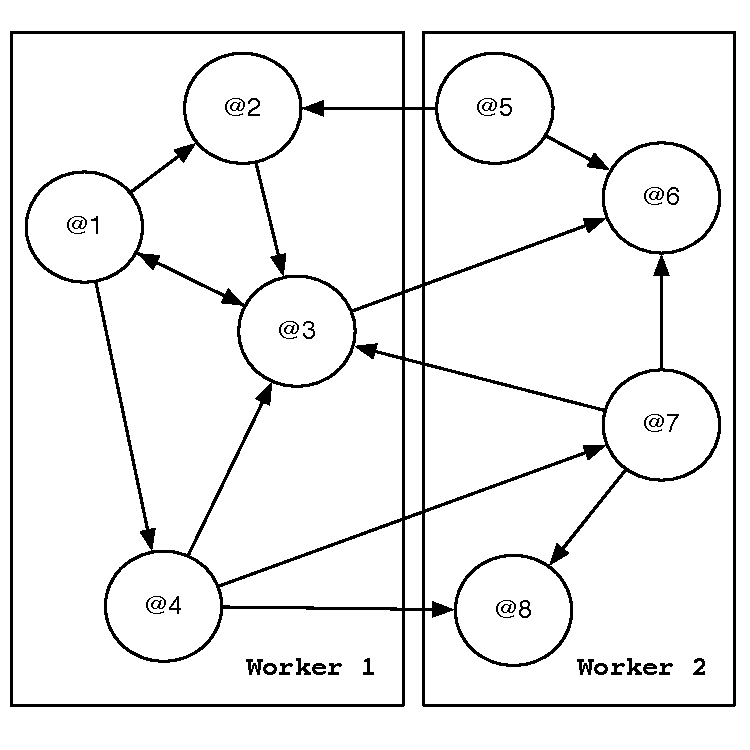
\includegraphics[height=7cm]{graph_coordination.pdf}
   \end{center}
\end{frame}


\subsection{Quick-Sort}

\begin{frame}[fragile]
  \frametitle{Quick-Sort}
  \begin{columns}[t]
       \column{.45\textwidth}
       \begin{block}{Program}
         \begin{Verbatim}[fontsize=\tiny,frame=single,commandchars=\\\{\}]
\alert[1]{down(@0, tosort).}

\alert[2]{down(A, [])}
   \alert[2]{-o up(A, []).}
\alert[2]{down(A, [X])}
   \alert[2]{-o up(A, [X]).}
\alert[2]{down(A, [X, Y]),}
\alert[2]{X < Y}
   \alert[2]{-o up(A, [X, Y]).}
\alert[2]{down(A, [X, Y]),}
\alert[2]{X >= Y}
   \alert[2]{-o up(A, [Y, X]).}
\alert[3]{down(A, [X | L])}
   \alert[3]{-o buildpivot(A, L, X, [], []).}
         \end{Verbatim}
      \end{block}
      \column{.5\textwidth}
      \begin{block}{Explanation}
         {\scriptsize
         \begin{itemize}
            \only<1>{\item The quick-sort program starts with a single node and dynamically builds the graph of nodes}
            \only<1>{\item A node receives an unsorted list in the second argument of \texttt{down/2} and must generate an \texttt{up/2} fact after sorting the list}
            \only<2>{\item In the base cases, the list can be immediately sorted}
            \only<3>{\item In the recursive case, we split the list...}
         \end{itemize}
         }
      \end{block}
   \end{columns}
\end{frame}

\begin{frame}[fragile]
  \frametitle{Quick-Sort}
  \begin{columns}[t]
       \column{.5\textwidth}
       \begin{block}{Program}
         \begin{Verbatim}[fontsize=\tiny,frame=single,commandchars=\\\{\}]
\alert[2]{buildpivot(A, [], X, Smaller, Greater)}
   \alert[2]{-o exists B, C. (back(B, A), down(B, Smaller),}
            \alert[2]{back(C, A), down(C, Greater),}
            \alert[2]{waitpivot(A, B, C, X)).}

\alert[1]{buildpivot(A, [Y | L], X, Smaller, Greater),}
\alert[1]{Y <= X}
   \alert[1]{-o buildpivot(A, L, X, [Y | Smaller], Greater).}
\alert[1]{buildpivot(A, [Y | L], X, Smaller, Greater),}
\alert[1]{Y > X}
   \alert[1]{-o buildpivot(A, L, X, Smaller, [Y | Greater]).}

\alert[3]{waitpivot(A, NodeSmaller, NodeGreater, Pivot),}
\alert[3]{sorted(A, NodeSmaller, Smaller),}
\alert[3]{sorted(A, NodeGreater, Greater)}
   \alert[3]{-o append(A, Smaller, [Pivot | Greater]).}
   
\alert[3]{up(A, L), back(A, B) -o sorted(B, A, L).}
         \end{Verbatim}
      \end{block}
      \column{.45\textwidth}
      \begin{block}{Explanation}
         {\scriptsize
         \begin{itemize}
            \only<1>{\item \texttt{buildpivot/4} will split the list: elements less or equal than \texttt{X} in the fourth argument and elements greater than \texttt{X} in the fifth argument}
            \only<2>{\item Once the list is split, we create nodes \texttt{B} and \texttt{C} that will sort the two sub-lists
            \item \texttt{waitpivot} is then used to wait for the sorted lists from \texttt{B} and \texttt{C}}
            \only<3>{\item Nodes \texttt{B} and \texttt{C} send a \texttt{sorted/3} fact to \texttt{A}
            \item Results are then appended and sent recursively to the root node}
         \end{itemize}
         }
      \end{block}
   \end{columns}
\end{frame}

\begin{frame}[fragile]
  \frametitle{Quick-Sort}
  \begin{block}{Example Execution}
     \begin{figure}
        \includegraphics<1>[height=4.5cm]{quicksort1.pdf}
        \includegraphics<2>[height=4.5cm]{quicksort2.pdf}
        \includegraphics<3>[height=4.5cm]{quicksort3.pdf}
        \includegraphics<4>[height=4.5cm]{quicksort4.pdf}
        \includegraphics<5>[height=4.5cm]{quicksort5.pdf}
     \end{figure}
  \end{block}
\end{frame}


\begin{frame}[fragile]
   \frametitle{Other uses of Linear Meld}
   \begin{itemize}
      \item Belief Propagation, Splash Belief Propagation
      \item Neural Networks
      \item MiniMax
      \item N-Queens
      \item PageRank
      \item Graph algorithms: shortest path, search, coloring, ...
   \end{itemize}
   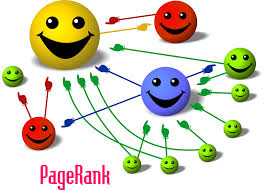
\includegraphics[height=4cm]{pagerank.jpeg}
   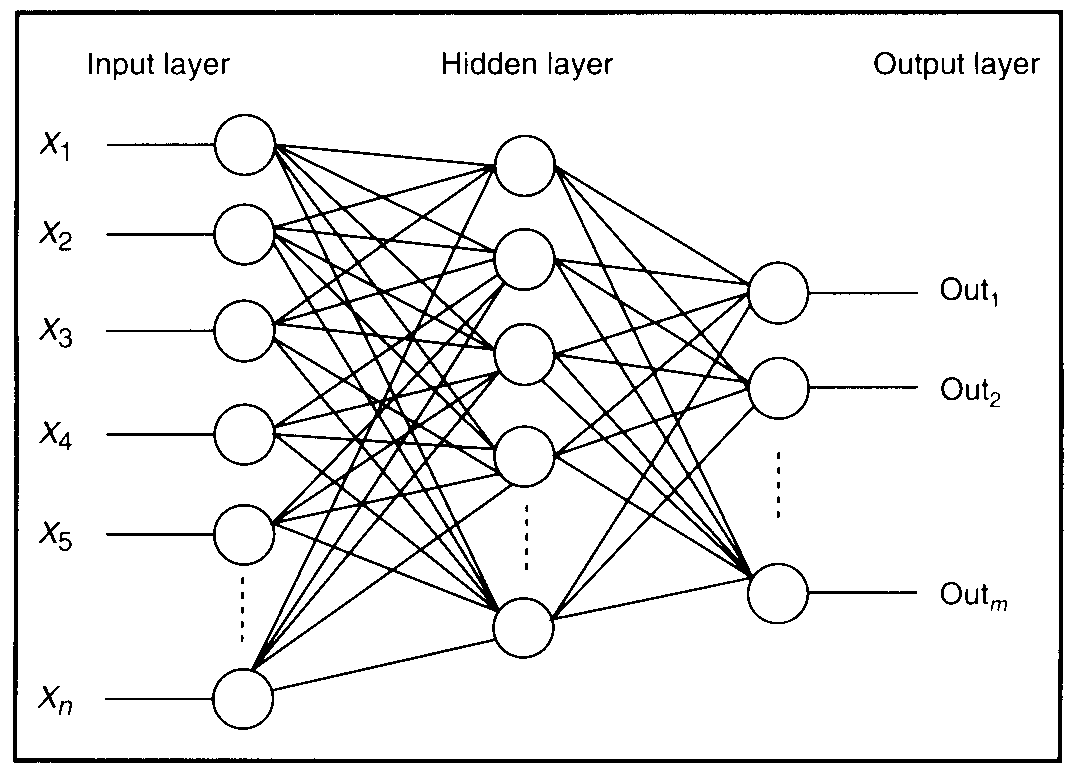
\includegraphics[height=4cm]{neural_networks.png}
\end{frame}


\newcommand{\mz}{\m{match} \;}
\newcommand{\tab}[0]{\;\;\;\;}
\newcommand{\dz}{\m{derive} \;}
\newcommand{\comp}[0]{\m{comp} \;}
\newcommand{\az}{\m{apply} \;}
\newcommand{\doz}{\m{run} \;}
\newcommand{\seqnocut}[3]{#1 ; #2 \Rightarrow #3}
\newcommand{\defeq}{\buildrel\triangle\over =}
\newcommand{\compr}[1]{\m{def} \; #1}

\newcommand{\mo}{\m{match}_1 \;}
\newcommand{\cont}{\m{cont} \;}
\newcommand{\contc}{\m{contc} \;}
\newcommand{\done}{\m{derive}_1 \;}
\newcommand{\doo}{\m{run}_1 \;}
\newcommand{\mc}[0]{\m{match}_c \; }
\newcommand{\dall}[0]{\m{fix} \; }
\newcommand{\strans}[0]{\m{strans} \;}
\newcommand{\dc}{\m{derive}_c \;}
\newcommand{\ao}{\m{apply}_1 \;}

We now present the sequent calculus of a fragment of intuitionistic linear
logic~\cite{girard-87} used by LM followed by the dynamic semantics built on top of
this fragment.

The fragment of linear logic used by LM is presented in \ref{linear_logic}.
We use a standard set of connectives except the $\m{def} \; A$ connective, which is used to logically justify comprehensions and aggregates.
The sequent calculus has the form $\Psi; \Gamma; \Delta \rightarrow C$, where $\Psi$ is the typed term context used in the quantifiers, $\Gamma$ is the set
of persistent terms, $\Delta$ is the multi-set of linear propositions and $C$ is the proposition we want to prove.
Table~\ref{table:linear} relates the linear logic directives with the LM syntax.


\footnotesize
\begin{center}
\begin{table}\resizebox{14cm}{!}{
    \begin{tabular}{ c l c l}
    \hline
    Connective                   & Description                                        & LM Place   & LM Example                           \\ \hline \hline
    $\emph{fact}(\hat{x})$       & Linear facts.                                      & Body/Head  & \texttt{path(A, P)}                  \\ 
    $\bang \emph{fact}(\hat{x})$ & Persistent facts.                                  & Body/Head  & \texttt{$\bang$edge(X, Y, W)}        \\ 
    $1$                          & Represents rules with an empty head.               & Head       & \texttt{1}                           \\ 
    $A \otimes B$                & Connect two expressions.                           & Body/Head  & \texttt{p(A), e(A, B)}               \\ 
    $\forall x. A$               & For variables defined in the rule.                 & Rule       & \texttt{p(A) $\lolli$ r(A)}          \\ 
    $\exists x. A$               & Instantiates new node variables.                   & Head       & \texttt{exists A.(p(A, P))}          \\ 
    $A \lolli B$                 & $\lolli$ means "linearly implies".                 & Rule       & \texttt{p(A, B) $\lolli$ r(A, B)}    \\ 
                                 & $A$ is the body and $B$ is the head.               &            &                                      \\ 
    $\m{def} A. B$               & Extension called definitions. Used for             & Head       & \texttt{\{B | !e(A, B) | v(B)\}}     \\ 
                                 & comprehensions and aggregates.                     &            &                                      \\ \hline
    \end{tabular}}
\caption{Connectives from Linear Logic used in LM.}
\label{table:linear}
\end{table}
\end{center}
\normalsize


For definitions, we took inspiration from Baelde's work on least and greatest fixed points in linear logic~\cite{Baelde:2012:LGF:2071368.2071370}. Baelde's system goes beyond
simple recursive definitions and allows proofs using induction and co-induction in linear logic. Fortunately, the proof system satisfies
cut-elimination~\cite{Baelde:2012:LGF:2071368.2071370} which makes it consistent.

In a comprehension, we want to apply an implication to as many matches as the database allows. One way to formally describe comprehensions would be to use persistent
rules that would be used a few times and then would be forgotten. A more reasonable approach is to use
definitions. Given a comprehension $C = \{ \; \widehat{x}; \; A; \; B \; \}$ with a body $A$ and a head $B$, then we can build the following recursive definition:

\[
\compr{C} \defeq 1 \with ((A \lolli B) \otimes \compr{C})
\]

We can unfold $\compr{C}$ to either stop (by selecting $1$) or get a new linear implication $A \lolli B$
to apply the comprehension once. Because we also get another $\compr{C}$ by selecting the right hand side,
the comprehension can be applied again, recursively.

This form of definition does not capture the desired \emph{maximality} aspect of the comprehension,
since it commits to finding a particular form of proof and not all possible proofs. The low level
operational semantics will ensure maximality.

Aggregates work identically, but they need an extra argument to accumulate the aggregated value. If a sum aggregate $C$ has the form $[\;\m{sum} \Rightarrow y; \; \widehat{x}; \; A; \; B_1; \; B_2 \;]$, then the definition will be as follows (the aggregate is initiated as $\compr{C} \; 0$):

\[
\compr{C} \; V \defeq (\lambda v. B_2)V \with (\forall x. ((Ax \lolli B_1) \otimes \compr{C} \; (x + V)))
\]

\subsection{Dynamic Semantics}

The high level dynamic semantics (HLD) formalize the mechanism of matching rules and deriving new facts and is closely related to the fragment presented above.
From the sequent calculus, we consider $\Gamma$ and $\Delta$ the database of persistent and linear facts, respectively.
We consider the rules of the program as persistent linear implications of the form $\bang (A \lolli B)$ that we put in a separate context $\Phi$.
We ignore the right hand side $C$ of the calculus and use inversion on the $\Delta$ and $\Gamma$ contexts so that we only have atomic terms (facts). To apply rules
we use chaining by focusing on the derivation rules of $\Phi$.

\scriptsize
\begin{figure}[h]

\[
\infer[\doz rule]
{\doz \Gamma ; \Delta ; R, \Phi \rightarrow \Xi' ; \Delta' ; \Gamma'}
{\az \Gamma ; \Delta ; R \rightarrow \Xi' ; \Delta' ; \Gamma'}
\]

\[
\infer[\az rule]
{\az \Gamma ; \Delta, \Delta'' ; A \lolli B \rightarrow \Xi' ; \Delta' ; \Gamma'}
{\mz \Gamma ; \Delta \rightarrow A & \dz \Gamma ; \Delta''; \Delta; \cdot ; \cdot ; B \rightarrow \Xi' ; \Delta' ; \Gamma'}
\]

\[
\infer[\mz 1]
{\mz \Gamma; \cdot \rightarrow 1}
{}
\tab
\infer[\mz p]
{\mz \Gamma; p \rightarrow p }
{}
\tab
\infer[\mz \bang p]
{\mz \Gamma, p; \cdot \rightarrow \bang p}
{}
\]

\[
\infer[\mz \otimes]
{\mz \Gamma; \Delta_1, \Delta_2 \rightarrow A \otimes B}
{\mz \Gamma; \Delta_1 \rightarrow A & \mz \Delta_2 \rightarrow B}
\]

\[
\infer[\dz p]
{\dz \Gamma ; \Delta ; \Xi ; \Gamma_1 ; \Delta_1 ; p, \Omega \rightarrow \Xi' ; \Delta' ; \Gamma'}
{\dz \Gamma ; \Delta ; \Xi ; \Gamma_1 ; p, \Delta_1 ; \Omega \rightarrow \Xi' ; \Delta' ; \Gamma'}
\tab
\infer[\dz \bang p]
{\dz \Gamma ; \Delta ; \Xi ; \Gamma_1 ; \Delta_1 ; \bang p, \Omega \rightarrow \Xi' ; \Delta' ; \Gamma'}
{\dz \Gamma ; \Delta ; \Xi ; \Gamma_1, p ; \Delta_1 ; \Omega \rightarrow \Xi' ; \Delta' ; \Gamma'}
\]

\[
\infer[\dz \otimes]
{\dz \Gamma ; \Delta ; \Xi ; \Gamma_1 ; \Delta_1 ; A \otimes B, \Omega \rightarrow \Xi' ; \Delta' ; \Gamma'}
{\dz \Gamma ; \Delta ; \Xi ; \Gamma_1 ; \Delta_1 ; A, B, \Omega \rightarrow \Xi' ; \Delta' ; \Gamma'}
\tab
\infer[\dz 1]
{\dz \Gamma ; \Delta ; \Xi ; \Gamma_1; \Delta_1 ; 1, \Omega \rightarrow \Xi' ; \Delta' ; \Gamma'}
{\dz \Gamma ; \Delta ; \Xi ; \Gamma_1; \Delta_1 ; \Omega \rightarrow \Xi' ; \Delta' ; \Gamma'}
\]

\[
\infer[\dz end]
{\dz \Gamma ; \Delta ; \Xi' ; \Gamma' ; \Delta' ; \cdot \rightarrow \Xi' ; \Delta' ; \Gamma'}
{}
\]


\[
\infer[\dz comp]
{\dz \Gamma ; \Delta ; \Xi ; \Gamma_1 ; \Delta_1 ; \comp A \lolli B, \Omega \rightarrow \Xi' ; \Delta' ; \Gamma'}
{\dz \Gamma ; \Delta ; \Xi ; \Gamma_1 ; \Delta_1 ; 1 \with (A \lolli B \otimes \comp A \lolli B), \Omega \rightarrow \Xi' ; \Delta' ; \Gamma'}
\]

\[
\infer[\dz \lolli]
{\dz \Gamma ; \Delta_a, \Delta_b ; \Xi ; \Gamma_1 ; \Delta_1 ; A \lolli B, \Omega \rightarrow \Xi' ; \Delta' ; \Gamma'}
{\mz \Gamma ; \Delta_a \rightarrow A & \dz \Gamma ; \Delta_b ; \Xi, \Delta_a ; \Gamma_1 ; \Delta_1 ; B, \Omega \rightarrow \Xi' ; \Delta' ; \Gamma'}
\]

\[
\infer[\dz \with L]
{\dz \Gamma ; \Delta ; \Xi ; \Gamma_1 ; \Delta_1 ; A \with B, \Omega \rightarrow \Xi' ; \Delta'; \Gamma'}
{\dz \Gamma ; \Delta ; \Xi ; \Gamma_1 ; \Delta_1 ; A, \Omega \rightarrow \Xi' ; \Delta'; \Gamma'}
\tab
\infer[\dz \with R]
{\dz \Gamma ; \Delta ; \Xi ; \Gamma_1 ; \Delta_1 ; A \with B, \Omega \rightarrow \Xi' ; \Delta' ; \Gamma'}
{\dz \Gamma ; \Delta ; \Xi ; \Gamma_1 ; \Delta_1 ; B, \Omega \rightarrow \Xi' ; \Delta' ; \Gamma'}
\]

\caption{High Level Dynamic Semantics.}
\label{hld_semantics}
\end{figure}
\normalsize

The HLD semantics are shown in Fig.~\ref{hld_semantics} and are composed of four judgments:
\begin{enumerate}
   \item $\doz \Gamma; \Delta; \Phi \rightarrow \Xi'; \Delta'; \Gamma'$ picks a rule from $\Phi$ and applies it using facts from $\Gamma$ and $\Delta$. $\Xi'$, $\Delta'$ and $\Gamma'$ are the outputs of the derivation process. $\Xi'$ are the linear facts consumed, $\Delta'$ are the linear facts derived and $\Gamma'$ the new persistent facts;
   \item $\az \Gamma; \Delta; R \rightarrow \Xi'; \Delta'; \Gamma'$ picks a subset of linear facts from $\Delta$ and matches the body of the rule $R$ and then derives the head;
   \item $\mz \Gamma; \Delta \rightarrow A$ verifies that $\Delta$ proves $A$ directly;
   \item $\dz \Gamma; \Delta; \Xi; \Gamma_1; \Delta_1, \Omega \rightarrow \Xi'; \Delta'; \Gamma'$ deconstructs and instantiates the ordered head terms $\Omega$ and adds them to $\Delta_1$ and $\Gamma_1$, the contexts for new linear and persistent facts, respectively.
\end{enumerate}

Comprehensions are derived by non-deterministically deciding to apply the comprehension ($\dz \with L$ and $\dz \with R$)
and then using the $\mz$judgment in the rule $\dz comp$. We note that the HLD semantics do not take distribution into account,
since we assume that the database is global. We also omit the quantifiers and do not deal with unification since it complicates the formal system.

The low level dynamic semantics (LLD) shown in \ref{low_level_semantics} improve upon HLD by adding rule priorities, by removing non-determinism
when matching the body of rules by modeling all the matching steps and by applying comprehensions or aggregates as many times as the database allows.

In LLD we try all the rules in order. For each rule, we use a \emph{continuation stack} to store the \emph{continuation frames} created by
each fact template $p$ present
in the body of the rule. Each frame considers all the facts relevant to the template given the current variable bindings ($\mo$rules), that
may or not fail during the remaining matching process. If we fail, we backtrack to try other alternatives (through $\cont$rules). If the
continuation stack becomes empty, we backtrack to try the next rule (rule $\cont next \; rule$). When we succeed the facts consumed are known
($\mo end$).

The derivation process in LLD is similar to the one used in HDL, except for the case of comprehensions or aggregates. For such cases
($\done comp$), we need to create a continuation stack and start matching the body of the construct as we did before.
When we match the body ($\mc$judgment), we fully derive the head ($\dc$judgment) and then we reuse the continuation stack to find which
other combinations of the database facts can be consumed ($\dc end$). By definition, the continuation stack contains
enough information to go through all combinations in the database.

However, in order to reuse the stack, we need to \emph{fix} it by removing all the frames pushed after the first continuation frame
of a linear fact. If we tried to use those frames, we would assumed that the linear facts used by the other frames were still in the database, but that
is not true because they have been consumed during the first application of the comprehension.
For example, if the body is $\bang\mathtt{a(X), b(X), c(X)}$ and the continuation stack has three frames (one per fact), we cannot backtrack to the frame of $\mathtt{c(X)}$
since at that point the matching process was assuming that the previous \texttt{b(X)} linear fact was still available.
Moreover, we also remove the consumed linear facts
from the frames of \texttt{b(X)} and $\bang$\texttt{a(X)} in order to make the stack fully consistent with the new database.
This is performed by rules using the $\strans$and $\dall$judgments.

We finally stop applying the comprehension when the continuation stack is empty ($\contc end$). 
Aggregates use the same mechanism as comprehensions, however we also need to keep track of the accumulated value.

\subsection{Soundness}

The soundness theorem proves that if a rule was successfully derived in the LLD semantics then it can also be derived in the HLD semantics. The completeness theorem cannot
be proven since LLD lacks the non-determinism inherent in HLD.

We prove that matching the body of a rule in LLD can also be performed in HLD (matching soundness) and that deriving the head of the rule is also sound (derivation soundness). The matching soundness uses induction on the size of the continuation frames, the size of the continuation stack and the size of terms to match to reconstitute a particular matching tree in HLD.

The derivation soundness lemma is trivial except for the case of comprehensions and aggregates. For such cases we use the matching soundness lemma applied $n$ times (for maximality) and then rebuild the derivation tree in HLD using $2 n$ matching and derivation judgments. These can be retrieved by applying
induction on size of the continuation stack and continuation frames.\footnote{Details can be
found in \url{https://github.com/flavioc/formal-meld/blob/master/doc.pdf?raw=true}.}

\begin{comment}
\subsubsection{Soundness}

The soundness theorem proves that if a rule was successfully derived in the LLD semantics then it can also be derived in the HLD semantics. The completeness theorem cannot
be proven since LLD lacks the non-determinism inherent in HLD.

The first main lemma of the soundness proof proves that if we can match the body
of a rule at the low level then we can also match the rule in the high level system using the same database.

\begin{lemma}[Body Match]
Given a match $\mo \Gamma; \Delta_1, \Delta_2; \cdot; A; B; \cdot; R \rightarrow \Xi'; \Delta'; \Gamma'$ that is related to $A$, $\Delta_1, \Delta_2$ and $\Gamma$, we get either:

\begin{enumerate}
   \item $\cont \cdot; B; R; \Gamma; \Xi'; \Delta'; \Gamma'$;
   \item $\mz \Delta_2 \rightarrow A$ and $\mo \Gamma; \Delta_1; \Delta_2; \cdot; B; C'; R \rightarrow \Xi'; \Delta'; \Gamma'$ (related)
\end{enumerate}
\end{lemma}
\begin{proof}Use the main matching soundness theorem.
\end{proof}

When we say that a match is related to a term $A$ and a database $\Delta_1, \Delta_2, \Gamma$ we mean that
the matching judgment is related to the body $A$ of a rule and the initial database is $\Delta_1, \Delta_2, \Gamma$, where $\Gamma$ are
the persistent facts, $\Delta_2$ the linear facts consumed to match the body and $\Delta_1$ the remaining linear facts.
Moreover, the continuation stack is related to $A$ and to the database, therefore it is consistent in relation to them.

The body match lemma tells us that if we start a match of a body $A$ we will either fail (1) and need to try another rule in $R$ or we succeed by building the high level matching judgment $\mz \Delta_2 \rightarrow A$ (the soundness result) and reaching the end of the matching process $\mo \Gamma; \Delta_1; \Delta_2; \cdot; B; C'; R \rightarrow \Xi'; \Delta'; \Gamma'$.

This lemma uses a more complicated theorem that is recursively defined through judgments $\m{match}_1$ and $\m{cont}$ that use mutual induction on the
size of the continuation stack, the size of the remaining terms to match and also the size of alternatives at each continuation frame. We always ensure that the
continuation stack stays consistent at all times, when backtracking or moving forward. Theorem is presented in Appendix~\ref{main_soundness_theorem}.
 
The second stepping stone in the soundness proof is the derivation lemma. After we successfully match
the body of a rule, we need to prove that the derivation process (through judgments $\m{derive}_1$)
is also sound. This lemma is as follows:

\begin{lemma}[Derivation]
   If $\done \Gamma; \Delta; \Xi; \Gamma_1; \Delta_1; \Omega \rightarrow \Xi'; \Delta'; \Gamma'$ then $\dz \Gamma; \Delta; \Gamma_1; \Delta_1; \Omega \rightarrow \Xi'; \Delta'; \Gamma'$.
\end{lemma}
\begin{proof}
   Straightforward use of induction on $\Omega$ (the terms of the head) except for the sub-case of comprehensions and aggregates, where we need to use the comprehension and aggregate theorems to construct the derivation tree using $n$ applications of the corresponding construct.
\end{proof}

In the case of proving the soundness of comprehensions, we use a very identical theorem to the one used
to prove the body match soundness. However, in this case we need to reuse the continuation stack several
times (as many as many comprehensions can be applied). Using induction on the continuation stack, we get
$n$ (where $n \ge 0$) applications of the comprehension and $n \; \m{match}$ and $n \; \m{derive}$ judgments
that can be used to rebuild the derivation tree at the low level by using the $\dz \with L$, $\dz \with R$
and $\dz \lolli$ rules to fold and unfold the comprehension term. The theorem for aggregates works similarly.
\end{comment}


\begin{frame}
   \frametitle{Conclusions}
   \begin{itemize}
      \item LM is easily ported to different distributed architectures
      \begin{itemize}
         \item Current implementation works on multicores
         \item Performance results are encouraging when compared against other imperative frameworks
         \item Programs are much shorter!
      \end{itemize}
      \item Graph problems are important and are here to stay
      \begin{itemize}
        \item Size of data will increase
        \item Implementations will be needed to run on very large graphs
      \end{itemize}
   \end{itemize}
\end{frame}

\begin{frame}{Thank You}
\begin{center}
{\Huge Thank you for your time!}
\end{center}
\end{frame}

\end{document}

